\chapter{Numbers}

\begin{quote}
God created the integers, the rest is the work of man.

\hfill---Leopold Kronecker 
\end{quote}

\section{The Integers}

In this course we will discuss several different sets of numbers. The
first set we encounter is called the \textit{integers}.

\begin{definition}\index{integers}\index{Z@$\Z$}
The set of whole numbers, zero, and negative whole numbers is called
the set of \textbf{integers}. We use the symbol $\Z$ to denote the
integers:
\[
\Z = \{\dots, -5,-4,-3,-2,-1,0,1,2,3,4,5,\dots \}
\]
\end{definition}

In case you're wondering, the symbol $\Z$ is used because
\textit{Zahlen} is the German word for ``numbers.'' 


\subsection{Addition}

Addition is probably the first operation we learn. 

\begin{question}
Write a story problem whose solution is given by the expression
$19+17$. Let this context be a ``working'' model for addition.
\end{question}
\QM

\begin{question}
Does your model show associativity of addition? If so, explain how. If
not, can you come up with a new model (story problem) that does?
\end{question}
\QM

\begin{question}
Does your model show commutativity of addition? If so, explain how. If
not, can you come up with a new model that does?
\end{question}
\QM


\begin{question}
Does your model work with negative integers, that is does it model say
$19+ (-17)$? If so, explain how. If not, can you come up with a new
model that does?
\end{question}
\QM


\begin{question}
We know that 
\[
a - b  = a + (-b),
\]
but I insist that the left-hand side of the equation is conceptually
different from the right-hand side of the equation. Write two story
problems, one solved by $19-17$ and the other solved by
$19+(-17)$. What's the difference? (Pun intended!)
\end{question}
\QM

\begin{teachingnote}
Here we are trying to have the students develop the ``take-away,''
along with the ``missing addend,'' and a ``comparison'' model for
subtraction.
\end{teachingnote}


\begin{question}
Can you use the two story problems above to model
\[
(-19)-17, \qquad  19 - (-17), \qquad (-19) - (-17)?
\]
\end{question}
\QM

\subsection{Multiplication}


Multiplication is more multifaceted than addition. 

\begin{question}
Write a story problem whose solution is given by the expression
$19\cdot 17$. Let this context be a ``working'' model for multiplication. 
\end{question}
\QM

\begin{teachingnote}
We would like to point out that the units used in addition are generally
the same for the different summands. However, with multiplication, the
different factors often have different units.
\end{teachingnote}



\begin{teachingnote}
The next question is with Problem~\ref{P:MA} of
Section~\ref{S:aritmetic} in mind. In particular to show
associativity, we suggest appealing to the notion of volume.
\end{teachingnote}

\begin{question}
Does your model show associativity of multiplication? If so, explain
how. If not, can you come up with a new model that does?
\end{question}
\QM

\begin{question}
Does your model show commutativity of multiplication? If so, explain
how. If not, can you come up with a new model that does?
\end{question}
\QM


\begin{question}
Does your model work with negative integers? In particular does your
model show that
\[
\text{positive}\cdot \text{negative} = \text{negative},
\]
\[
\text{negative}\cdot \text{positive} = \text{negative},
\]
and 
\[
\text{negative}\cdot \text{negative} = \text{positive}?
\]
If so, explain how. If not, can you come up with a new model that
does?
\end{question}
\QM

\begin{teachingnote}
This is difficult. The students may not be able to come up with a
model that works. This is OK---as this issue is addressed in
Problem~\ref{P:NNP}.
\end{teachingnote}


\subsection{Division} 

While addition and multiplication are good operations, the real
``meat'' of the situation comes with division.


\begin{definition}\index{divides}  %  \index{dn@$d "| n$}
We say that an integer $d$ \textbf{divides} an integer $n$ if there is
an integer $q$
\[
n = dq
\]
in this case we write $d | n$, which is said: ``$d$ divides $n$.'' 
\end{definition}

While this may seem easy, it is actually quite tricky. You must always
remember the following synonyms for \textit{divides}:
\[\index{multiple}\index{factor}
\text{``$d$ \textbf{divides} $n$''}\leftrightsquigarrow \text{``$d$ is
  a \textbf{factor} of $n$''}\leftrightsquigarrow \text{``$n$ is a
  \textbf{multiple} of $d$''}
\]


\begin{activitynote}
Activity \ref{A:dm} complements this section well.  % What Can Division Mean
\end{activitynote}



\begin{definition}\index{prime number} 
A \textbf{prime} number is a positive integer with exactly two
positive divisors, namely $1$ and itself.
\end{definition}

\begin{definition}\index{composite number} 
A \textbf{composite} number is a positive integer with more than two
positive divisors.
\end{definition}

I claim that every composite number is divisible by a prime number. Do
you believe me? If not, consider this:
\begin{quote}
Suppose there was a composite number that was \textit{not} divisible
by a prime. Then there would necessarily be a \textit{smallest}
composite number that is not divisible by a prime. Since this number
is composite, this number is the product of two even smaller numbers,
both of which have prime divisors. Hence our original number must have
prime divisors.
\end{quote}
\begin{question} 
What the heck just happened?! Can you rewrite the above paragraph,
drawing pictures and/or using symbols as necessary, making it more
clear?
\end{question}
\QM


\begin{activitynote}
Activity \ref{A:Pr} complements this section well.  %  There's Always Another Prime
\end{activitynote}


\subsection{Factoring}

At this point we can factor any composite completely into primes. To
do this, it is often convenient to make a \textit{factor
  tree}:\index{factor tree}

\[
\xymatrix@R=0pt@C=10pt{
  & 360 \ar@{-}[dl] \ar@{-}[dr] & & & & &\\
2 &     & 180 \ar@{-}[dl] \ar@{-}[dr] & & & & \\ 
  &  2   &     & 90 \ar@{-}[dl] \ar@{-}[dr] & & & \\
  &      &  2  &    & 45  \ar@{-}[dl] \ar@{-}[dr] & & \\ 
  &      &     & 5  &    & 9 \ar@{-}[dl] \ar@{-}[dr] &\\ 
  &      &     &    &  3  &  & 3
}
\]

From this tree\footnote{Why is this a tree? It looks more like roots to me!} we see that
\[
360 = 2^3 \cdot 3^2 \cdot 5.
\]

At each step we simply divided by whichever prime number seemed most
obvious, branched off the tree and kept on going. From our factor
tree, we can see some of the divisors of the integer in
question. However, there are many composite factors that can be built
up from the prime divisors. One of the most important is the
\textit{greatest common divisor}.

\begin{definition}\index{GCD}\index{greatest common divisor} 
The \textbf{greatest common divisor} (GCD) of two numbers $a$ and $b$
is a number $g = \gcd(a,b)$ where:
\begin{enumerate}
\item $g|a$ and $g|b$.
\item If $d|a$ and $d|b$, then $d \le g$.
\end{enumerate}
\end{definition}

\begin{question}
How do you use a factor tree to compute the GCD of two integers?
\end{question}
\QM



So, to factor an integer or find the GCD, one could use a factor
tree. However, when building the factor tree, we had to know what
primes to divide by. What if no prime comes to mind? What if you want
to factor the integer $391$ or $397$? This raises a new question:

\begin{question} 
How do you check to see if a given integer is prime? What possible
divisors must you check? When can you stop checking?
\end{question}
\QM


\begin{activitynote}
Activity \ref{A:Sie} complements this section well. % Sieving It All Out
\end{activitynote}


%\begin{question}
%How should you identify all the primes between $1$ and $100$? Big
%hint: Maybe you should either go to the shoe store, or read up on
%Eratosthenes.\index{Eratosthenes}
%\end{question}
%\QM







\subsection{Division with Remainder}


We all remember long division\index{long division}, or at least we
remember \textit{doing} long division. Sometimes, we need to be
reminded of our \textit{forgotten foes}\index{forgotten foes}. When
aloof old Professor Rufus was trying to explain division to his class,
he merely wrote
\[
d\,\begin{tabular}[b]{@{}r@{} r}
$q$ &\, R\,$r$\\ \cline{1-1}
\big)\begin{tabular}[t]{@{}l@{}}
$n$ 
\end{tabular}
\end{tabular}
\qquad\text{where}\qquad
\begin{tabular}{l}
$d$ is the divisor \\ \index{divisor}
$n$ is the dividend \\ \index{dividend}
$q$ is the quotient \\ \index{quotient}
$r$ is the remainder \index{remainder}
\end{tabular}
\]
and walked out of the room.

\begin{question} 
Can you give $3$ much needed examples of long division with
remainders?
\end{question}
\QM

\begin{question} 
Given positive integers $d$, $n$, $q$, and $r$ how do you know if they
leave us with a correct expression above?
\end{question}
\QM

\begin{question} 
Given positive integers $d$ and $n$, how many different sets of $q$
and $r$ can you find that will leave us with a correct expression
above?
\end{question}
\QM


The innocuous questions above can be turned into a theorem. We'll start
it for you, but you must finish it off yourself:

\begin{theorem}[Division Theorem]\index{Division Theorem!for integers}
Given any integer $n$ and a nonzero integer $d$, there exist unique
integers $q$ and $r$ such that
\vspace{1in}
\end{theorem}
\noindent The above space has intentionally been left blank for you to
fill in.


\begin{teachingnote}
Here we want the students to realize that
\[
n = dq + r\qquad\text{where } 0 \le r < d 
\]
\end{teachingnote}


Now consider the following picture:
\[
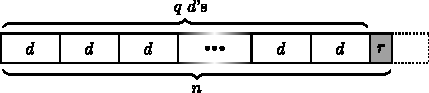
\includegraphics{../graphics/divisionThmProof.pdf}
\]
\begin{question} 
How does the picture above ``prove'' the Division Theorem for positive
integers? How must we change the picture if we allow negative values
for $n$ and $d$?
\end{question}
\QM

\begin{teachingnote}
The second part of this question might be too hard for most students.
\end{teachingnote}




\begin{activitynote}
Activity \ref{A:CF} complements this section well.  % There Are Many Factors to Consider
\end{activitynote}


\newpage


\begin{problems}
\begin{enumerate}
\item Describe the set of integers. Give some relevant and revealing
  examples/nonexamples.
\item Explain how to model integer addition with pictures or
  items. What relevant properties should your model show?
\item Explain how to model integer multiplication with pictures or
  items. What relevant properties should your model show?
\item Explain what it means for one integer to \textit{divide} another
  integer. Give some relevant and revealing examples/nonexamples.
\item Use the definition of \textit{divides} to decide whether the
  following statements are true or false. In each case, a detailed
  argument and explanation must be given justifying your claim.
\begin{enumerate}
\item $5|30$
\item $7|41$
\item $6|(2^2\cdot 3^4\cdot 5 \cdot 7)$
\item $1000|(2^7\cdot 3^9\cdot 5^{11}\cdot 17^8)$
\item $6000|(2^{21}\cdot 3^{17}\cdot 5^{89}\cdot 29^{20})$
\end{enumerate}
\item \textit{Incognito's Hall of Shoes} is a shoe store that just
  opened in Myrtle Beach, South Carolina. At the moment, they have 100
  pairs of shoes in stock. At their grand opening 100 customers showed
  up. The first customer tried on every pair of shoes, the second
  customer tried on every 2nd pair, the third customer tried on every
  3rd pair, and so on until the 100th customer, who only tried on the
  last pair of shoes.
\begin{enumerate}
\item Which shoes were tried on by only 1 customer?
\item Which shoes were tried on by exactly 2 customers?
\item Which shoes were tried on by exactly 3 customers?
\item Which shoes were tried on by the most number of customers?
\end{enumerate}
Explain your reasoning.
\item Factor the following integers:
\begin{enumerate}
\item $111$
\item $1234$
\item $2345$
\item $4567$
\item $111111$
\end{enumerate}
In each case, how large of prime must you check before you can be sure
of your answers? Explain your reasoning.
\item Explain how to deduce whether the following numbers are prime in
  as few calculations as possible:
\[
29 \qquad 53 \qquad 101 \qquad 359 \qquad 779 \qquad 839 \qquad 841
\]
In each case, describe precisely which computations are needed and
why those are the only computations needed.
\item Suppose you were only allowed to perform at most $7$
  computations to see if a number is prime. How large a number could
  you check?  Explain your reasoning.
\item Find examples of integers $a$, $b$, and $c$ such that $a \mid
  bc$ but $a\nmid b$ and $a\nmid c$. Explain your reasoning.
\item Can you find at least $5$ composite integers in a row? What
  about at least $6$ composite integers? Can you find $7$?
  What about $n$?  Explain your reasoning. Hint: Consider something
  like $5! = 5\cdot 4 \cdot 3 \cdot 2 \cdot 1$.
\item Use the definition of the \textit{greatest common divisor} to
  find the GCD of each of the pairs below. In each
  case, a detailed argument and explanation must be given justifying
  your claim.
\begin{enumerate}
\item $\gcd(462,1463)$
\item $\gcd(541,4669)$ 
\item $\gcd(10000,2^5\cdot 3^{19}\cdot 5^7\cdot 11^{13})$
\item $\gcd(11111,2^{14}\cdot 7^{21}\cdot 41^{5}\cdot 101)$
\item $\gcd(437^5,8993^3)$
\end{enumerate}

\item Lisa wants to make a new quilt out of $2$ of her favorite
  sheets. To do this, she is going to cut each sheet into as large of
  squares as possible while using the entire sheet and using whole
  inch measurements. 
\begin{enumerate}
\item If the first sheet is $72$ inches by $60$ inches what size
  squares should she cut? 
\item If the second sheet is $80$ inches by $75$ inches, what size
  squares should she cut? 
\item How she might sew these squares together? 
\end{enumerate}
Explain your reasoning.
\item Deena and Doug like to feed birds. They want to put 16 cups of
  millet seed and 24 cups of sunflower seeds in their feeder.
\begin{enumerate}
\item How many total scoops of seed (millet or sunflower) are required
  if their scoop holds 1 cup of seed?
\item How many total scoops of seed (millet or sunflower) are required
  if their scoop holds 2 cups of seed?
\item How large should the scoop be if we want to minimize the total
  number of scoops?
\end{enumerate}
Explain your reasoning.
\item Consider the expression:
\[
d\,\begin{tabular}[b]{@{}r@{} r}
$q$ &\, R\,$r$\\ \cline{1-1}
\big)\begin{tabular}[t]{@{}l@{}}
$n$ 
\end{tabular}
\end{tabular}
\qquad\text{where}\qquad
\begin{tabular}{l}
$d$ is the divisor \\
$n$ is the dividend \\
$q$ is the quotient \\
$r$ is the remainder
\end{tabular}
\]
\begin{enumerate}
\item Give $3$ relevant and revealing examples of long division with
  remainders.
\item Given positive integers $d$, $n$, $q$, and $r$ how do you know
  if they leave us with a correct expression above?
\item Given positive integers $d$ and $n$, how many different sets of
  $q$ and $r$ can you find that will leave us with a correct
  expression above?
\item Give $3$ relevant and revealing examples of long division with
  remainders where some of $d$, $n$, $q$, and $r$ are negative.
\item Still allowing some of $d$, $n$, $q$, and $r$ to be negative,
  how do we know if they leave us with a correct expression above?
\end{enumerate}
\item State the \textit{Division Theorem} for integers. Give some
  relevant and revealing examples of this theorem in action.
\item Explain what it means for an integer to \textit{not} divide
  another integer. That is, explain symbolically what it should mean
  to write:
\[
a \nmid b
\]
\item Consider the following:
\begin{align*}
20 \div 8 &= 2 \text{ remainder }4, \\
28 \div 12 &= 2 \text{ remainder }4.
\end{align*}
Is it correct to say that $20 \div 8 = 28 \div 12$? Explain your reasoning.
%\item Explain how if 
%\[
%n = dq_0 + r_0
%\]
%and $r_0> d$, you can find new $q$ and $r$ such that $n = dq+r$ and
%$0\le r< d$.
\item Give a formula for the $n$th even number. Show-off your formula
  with some examples.
\item Give a formula for the $n$th odd number. Show-off your formula
  with some examples.
\item Give a formula for the $n$th multiple of $3$. Show-off your
  formula with some examples.
\item Give a formula for the $n$th multiple of $-7$. Show-off your
  formula with some examples.
\item Give a formula for the $n$th number whose remainder when divided
  by $5$ is $1$. Show-off your formula
  with some examples.

\item Explain the rule
\[
\text{even} + \text{even} = \text{even}
\]
in two different ways. First give an explanation based on
pictures. Second give an explanation based on algebra. Your
explanations must be general, not based on specific examples.
\item Explain the rule
\[
\text{odd} + \text{even} = \text{odd}
\]
in two different ways. First give an explanation based on
pictures. Second give an explanation based on algebra.  Your
explanations must be general, not based on specific examples.
\item Explain the rule
\[
\text{odd} + \text{odd} = \text{even}
\]
in two different ways. First give an explanation based on
pictures. Second give an explanation based on algebra. Your
explanations must be general, not based on specific examples.
\item Explain the rule
\[
\text{even} \cdot \text{even} = \text{even}
\]
in two different ways. First give an explanation based on
pictures. Second give an explanation based on algebra. Your
explanations must be general, not based on specific examples.
\item Explain the rule
\[
\text{odd} \cdot \text{odd} = \text{odd}
\]
in two different ways. First give an explanation based on
pictures. Second give an explanation based on algebra. Your
explanations must be general, not based on specific examples.
\item Explain the rule
\[
\text{odd} \cdot \text{even} = \text{even}
\]
in two different ways. First give an explanation based on
pictures. Second give an explanation based on algebra. Your
explanations must be general, not based on specific examples.
\item Let $a\ge b$ be positive integers with $\gcd(a,b) =1$. Compute
  $\gcd(a +b, a-b)$. Explain your reasoning. Hints: 
\begin{enumerate}
\item Make a chart.
\item If $g|x$ and $g|y$ explain why $g|(x+y)$.
\end{enumerate}
\item Make a chart listing all pairs of positive integers whose
  product is $18$. Do the same for $221$, $462$, and $924$. Use this
  experience to help you explain why when factoring a number $n$, you
  only need to check factors less than or equal to $\sqrt{n}$.
\item \label{P:NNP}Matt is a member of the Ohio State University
  Marching Band. Being rather capable, Matt can take $x$ steps of size
  $y$ inches for all integer values of $x$ and $y$.  If $x$ is
  positive it means \textit{face North and take $x$ steps.} If $x$ is
  negative it means \textit{face South and take $|x|$ steps.} If $y$
  is positive it means your step is a \textit{forward step of $y$
    inches.} If $y$ is negative it means your step \textit{is a
    backward step of $|y|$ inches.}
\begin{enumerate}
\item Discuss what the expressions $x \cdot y$ means in this
  context. In particular, what happens if $x = 1$? What if $y=1$?
\item Using the context above, write and solve a word problem that
  demonstrates the rule:
\[
\text{negative}\cdot \text{positive} = \text{negative}
\]
Clearly explain how your problem shows this.
\item Using the context above, write and solve a word problem that
  demonstrates the rule:
\[
\text{negative}\cdot \text{negative} = \text{positive}
\]
Clearly explain how your problem shows this.
\end{enumerate}
\item Stewie decided to count the pennies he had in his piggy bank. He
  decided it would be quicker to count by fives. However, he ended
  with two uncounted pennies. So he tried counting by twos but ended
  up with one uncounted penny. Next he counted by threes and then by
  fours, each time there was one uncounted penny. Though he knew he
  had less than a dollars worth of pennies, and more than 50 cents, he
  still didn't have an exact count. Can you help Stewie out? Explain
  your reasoning.
\end{enumerate}
\end{problems}














\section{The Euclidean Algorithm}\index{Euclidean algorithm}\label{S:EA}


Up to this point, computing the GCD of two integers required you to
factor both numbers.  This can be difficult to do. The following
algorithm, called the \textit{Euclidean algorithm}, makes finding
GCD's quite easy. With that said, algorithms can be tricky to
explain. Let's try this---study the following calculations, they are
examples of the Euclidean algorithm in action:
\begin{align*}
22 &= \boldsymbol{6}\cdot 3 + \boldsymbol{4}\\ 
\boldsymbol{6} &= \boldsymbol{4}
\cdot 1 + \fbox{$\boldsymbol{2}$}\\ 4 &= 2 \cdot 2 + 0 \qquad 
\fbox{$\therefore \gcd(22,6) = 2$}
\end{align*}

\begin{align*}
33 &= \boldsymbol{24}\cdot 1 + \boldsymbol{9}\\
\boldsymbol{24} &= \boldsymbol{9} \cdot 2 + \boldsymbol{6}\\
\boldsymbol{9} &= \boldsymbol{6} \cdot 1 + \fbox{$\boldsymbol{3}$}\\
6 &= 3 \cdot 2 + 0 \qquad \fbox{$\therefore \gcd(33,24) = 3$} 
\end{align*}

\begin{align*}
42 &= \boldsymbol{16}\cdot 2 + \boldsymbol{10}\\
\boldsymbol{16} &= \boldsymbol{10} \cdot 1 + \boldsymbol{6}\\
\boldsymbol{10} &= \boldsymbol{6} \cdot 1 + \boldsymbol{4}\\
\boldsymbol{6} &= \boldsymbol{4} \cdot 1 + \fbox{$\boldsymbol{2}$}\\
4 &= 2 \cdot 2 + 0 \qquad \fbox{$\therefore \gcd(42,16) = 2$} 
\end{align*}

\begin{question}
Can you describe how to do the Euclidean algorithm?
\end{question}
\QM

\begin{question}
Can you explain why the Euclidean algorithm will always stop? Hint:
Division Theorem.
\end{question}
\QM



\begin{activitynote}
Activity \ref{A:GCDwork} complements this section well.  % Why Does It Work? 
\end{activitynote}


The algorithm demonstrated above is called the \textit{Euclidean
  algorithm} or \textit{Euclid's algorithm} because
Euclid\index{Euclid} uses it several times in Books VII and X of his
book \textit{The Elements}. Donald Knuth\index{Knuth} gives a
description of the Euclidean algorithm in the first volume of his
series of books \textit{The Art of Computer Programming}. Given
integers $m$ and $n$, he describes it as follows:
\begin{quote}
\begin{enumerate} 
\item\label{A:E1} [Find remainder.] Divide $m$ by $n$ and let $r$ be the remainder. (We will have $0\le r< n$.)
\item{[Is it zero?]} If $r=0$, the algorithm terminates; $n$ is the answer.
\item{[Interchange.]} Set $m \leftarrow n$, $n \leftarrow r$, and go
  back to step \ref{A:E1}.
\end{enumerate}
\end{quote}

\begin{question}
What do you think of this description? How does it compare to your
description of the Euclidean algorithm?
\end{question}
\QM

While the Euclidean algorithm is handy and fun, its real power is that
it helps us solve equations. Specifically it helps us solve
\textit{linear Diophantine equations}.

\begin{definition}\index{Diophantine equation}
A \textbf{Diophantine equation} is an equation where only integer
solutions are deemed acceptable.
\end{definition}

We're going to solve \textit{linear Diophantine equations}, that is, equations of the form:
\[
ax + by = c
\]
where $a$, $b$, and $c$ are integers and the only solutions we will
accept are also integers. Let's study the following calculations:

\begin{tabular}{lr}
\begin{minipage}{15em}
{\begin{align*}
22 &= 6\cdot 3 + 4 &\Leftrightarrow & &  22-6\cdot 3 &= \boldsymbol{4}\\ 
6 &= 4\cdot 1 + 2 &\Leftrightarrow  & &  6 - \boldsymbol{4}\cdot 1 &= 2\\ 
4 &= 2 \cdot 2 + 0 
\end{align*}}
\end{minipage}
&
\begin{minipage}{15em}
{\begin{align*}
6 - 4\cdot 1 &= 2 \\
6 - (22-6\cdot 3)\cdot 1 &= 2 \\
6\cdot 4 + 22(-1) &= 2 
\end{align*}}
\end{minipage} \\
\multicolumn{2}{c}{\fbox{$\therefore 22x + 6y =2$ where $x = -1$ and $y = 4$}}
\end{tabular}

\begin{tabular}{lr}
\begin{minipage}{15em}
{\begin{align*}
33 &= 24\cdot 1 + 9 & \Leftrightarrow & & 33 - 24\cdot 1 &= \boldsymbol{9}\\
24 &= 9 \cdot 2 + 6 & \Leftrightarrow & & 24 - \boldsymbol{9}\cdot 2 &= \boldsymbol{6}\\
9 &= 6 \cdot 1 + 3 & \Leftrightarrow & & 9 - \boldsymbol{6} \cdot 1  &= 3\\
6 &= 3 \cdot 2 + 0  
\end{align*}}
\end{minipage}
&
\begin{minipage}{15em}
{\begin{align*}
9 - 6 \cdot 1  &= 3 \\
9 - (24 - 9\cdot 2) \cdot 1  &= 3 \\
9\cdot 3 +  24\cdot(-1)  &= 3 \\
(33 - 24\cdot 1)\cdot 3 +  24\cdot(-1)  &= 3 \\
33\cdot 3 + 24\cdot (-4) &=3
\end{align*}}
\end{minipage} \\
\multicolumn{2}{c}{\fbox{$\therefore 33x + 24y =3$ where $x = 3$ and $y = -4$}}
\end{tabular}


\begin{question} 
Can you explain how to solve Diophantine equations of the form
\[
ax + by = g
\]
where $g = \gcd(a,b)$?
\end{question}
\QM


\subsection{Fundamental Theorems}



\begin{teachingnote}
An important point of this section is to make the student think about
the distributive property. One should try to point out each time
\[
a(x+y) = ax + ay
\]
occurs.
\end{teachingnote}


\begin{activitynote}
Activity \ref{A:Prome} complements this section well.  % Prome Factorization
\end{activitynote}

The Euclidean algorithm is also useful for theoretical
questions.

\begin{question} 
Given integers $a$ and $b$, what is the smallest positive integer that
can be expressed as
\[
ax + by
\]
where $x$ and $y$ are also integers?
\end{question}

I'm feeling chatty, so I'll take this one. I claim that $g =
\gcd(a,b)$ is the smallest positive integer that can be
expressed as
\[
ax + by
\]
where $x$ and $y$ are integers. How do I know? Well, suppose there was
a smaller positive integer, say $s$ where:
\[
ax + by = s
\]
Hmmm\dots but we know that $g|a$ and $g|b$. This means that $g$
divides the left-hand-side of the equation. This means that $g$
divides the right-hand-side of the equation. So $g|s$---but this is
impossible, as $s< g$. Thus $g$ is the smallest integer that can be
expressed as $ax +by$.


Believe it or not, we're going somewhere with all this. The next
\textit{lemma}\index{lemma} will help us out.  What is a lemma, you
ask? A lemma is nothing but a little theorem that helps us solve
another problem. Note that a lemma should not be confused with the
more sour \index{lemon|see{lemma}}\textit{lemon}, as that is something
different and unrelated to what we are discussing.

\begin{lemma}[Euclid's Lemma]\index{Euclid's Lemma} 
If $p$ is a prime number and $a$ and $b$ are integers
\[
p|ab \qquad\text{implies that} \qquad p | a\text{ or } p|b.
\]
\end{lemma}

\begin{question} Can you use the ideas above to explain why this lemma is true?
\end{question}
\QM



\begin{question} If $11 | 50a$, is it true that $11|a$?
\end{question}
\QM




Now we have set the stage for our fundamental theorem---it is
sometimes called the \textit{Fundamental Theorem of Arithmetic}:


\begin{theorem}[Unique Factorization]\index{Unique Factorization Theorem}\index{Fundamental Theorem!of Arithmetic}
Every integer greater than 1 can be factored uniquely (up to ordering)
into primes.
\end{theorem}

\begin{proof}
Well, if an integer is prime, we are done. If an integer is composite,
then it is divisible by a prime number. Divide and repeat with the
quotient. If our original integer was $n$, we'll eventually get:
\[
n = p_1p_2 \cdots p_m
\]
where some of the $p_i$'s may be duplicates. 

How do we know this factorization is unique? Well, suppose that
\[
n = p_1p_2 \cdots p_m = q_1q_2\cdots q_l
\]
where the $p_i$'s are all prime and none of them equal any of the
$q_j$'s which are also prime. So, $\gcd(p_1,q_1) = 1$, and by the
definition of ``divides''
\[
p_1 |q_1(q_2\cdots q_l).
\]
So by Euclid's Lemma, $p_1$ must divide $(q_2\cdots q_l)$. Repeat this
enough times and you will find that $p_1 = q_j$ for one of the $q_j$'s
above. Repeat this process for the $p_i$'s and you see that the
factorization is unique.
\end{proof}

\begin{question} 
Huh?! Can you explain what just happened drawing pictures and/or using
symbols as necessary? Could you also give some examples?
\end{question}
\QM

\begin{question} 
Thinking about Unique Factorization of the Integers, explain why it
makes sense to exclude $1$ from the prime numbers.
\end{question}
\QM


\begin{question} 
Thinking about Unique Factorization of the Integers, what must be the
case when a number ends in a $0$?
\end{question}
\QM



\newpage

\begin{problems}

\begin{enumerate}
\item Explain what a \textit{Diophantine equation} is. Give an example
  and explain why such a thing has real-world applications.
\item Explain what the GCD of two integers is. Give some relevant and
  revealing examples/nonexamples.
\item Explain what the LCM of two integers is. Give some relevant and
  revealing examples/nonexamples.
\item Use the Euclidean algorithm to find: $\gcd(671,715)$,
  $\gcd(667,713)$, $\gcd(671,713)$, $\gcd(682,715)$, $\gcd(601,735)$,
  and $\gcd(701,835)$.
\item Explain the advantages of using the Euclidean algorithm to find
  the GCD of two integers over factoring.
\item Find integers $x$ and $y$ satisfying the following Diophantine
  equations:
\begin{enumerate}
\item $671x + 715 y = 11$ 
\item $667x + 713 y = 69$ 
\item $671x + 713 y = 1$
\item $682x + 715 y = 55$
\item $601x + 735 y = 4$
\item $701x + 835 y = 15$
\end{enumerate}
\item Given integers $a$, $b$, and $c$, explain how you know when a
  solution to a Diophantine equation of the form
\[
ax + by = c
\]
exists.
\item Consider the Diophantine equation:
\[
15x + 4y = 1
\]
\begin{enumerate}
\item Use the Euclidean Algorithm to find a solution to this
  equation. Explain your reasoning.
\item Compute the slope of the line $15x + 4y = 1$ and write it in
  lowest terms. Show your work.
\item Plot the line determined by $15x + 4y = 1$ on graph paper.
\item Using your plot and the slope of the line, explain how to find
  $10$ more solutions to the Diophantine equation above.
\end{enumerate}
\item Explain why a Diophantine equation 
\[
ax + by = c
\]
has either an infinite number of solutions or zero solutions.
\item Josh owns a box containing beetles and spiders. At the moment,
  there are $46$ legs in the box. How may beetles and spiders are
  currently in the box? Explain your reasoning.
\item How many different ways can thirty coins (nickles, dimes, and
  quarters) be worth five dollars? Explain your reasoning.
\item Lisa collects lizards, beetles and worms. She has more worms
  than lizards and beetles together. Altogether in the collection
  there are twelve heads and twenty-six legs. How many lizards does
  Lisa have?  Explain your reasoning.
\item Can you make exactly \$$5$ with exactly $100$ coins assuming you
  can only use pennies, dimes, and quarters? If so how, if not why
  not?  Explain your reasoning.
\item A merchant purchases a number of horses and bulls for the sum
  of $1770$ talers. He pays $31$ talers for each bull, and $21$ talers
  for each horse. How many bulls and how many horses does the merchant
  buy? Solve this problem, explain what a \textit{taler} is, and
  explain your reasoning---note this problem is an old problem by
  L.\ Euler, it was written in the $1700$'s.
\item A certain person buys hogs, goats, and sheep, totaling $100$
  animals, for $100$ crowns; the hogs cost him $3\frac{1}{2}$ crowns
  a piece, the goats $1\frac{1}{3}$ crowns, and the sheep go for
  $\frac{1}{2}$ crown a piece. How many did this person buy of each?
  Explain your reasoning---note this problem is an old problem from
  \textit{Elements of Algebra} by L.\ Euler, it was written in the
  $1700$'s.
\item How many zeros are at the end of the following numbers:
\begin{enumerate}
\item $2^2 \cdot 5^8 \cdot 7^3\cdot 11^5$
\item $11!$
\item $27!$
\item $99!$
\item $1001!$
\end{enumerate}
In each case, explain your reasoning.
\item Decide whether the following statements are true or false. In
  each case, a detailed argument and explanation must be given
  justifying your claim.
\begin{enumerate}
\item $7|56$
\item $55|11$
\item $3|40$
\item $100 | (2^4\cdot 3^{17} \cdot 5^2\cdot 7)$
\item $5555 | (5^{20}\cdot 7^9\cdot 11^{11}\cdot 13^{23})$ 
\item $3| (3+ 6 + 9 + \cdots +300 + 303)$
\end{enumerate}
\item Suppose that 
\[
(3^5 \cdot 7^9 \cdot 11^x \cdot 13^y) | (3^a \cdot 7^b \cdot 11^{19} \cdot 13^7)
\]
What values of $a$, $b$, $x$ and $y$, make true statements? Explain
your reasoning.
\item Decide whether the following statements are true or false. In
  each case, a detailed argument and explanation must be given
  justifying your claim.
\begin{enumerate}
\item If $7|13a$, then $7|a$.
\item If $6|49a$, then $6|a$. 
\item If $10|65a$, then $10|a$.
\item If $14|22a$, then $14|a$.
\item $54|931^{21}$.
\item $54|810^{33}$.
\end{enumerate}
\item Joanna thinks she can see if a number is divisible by 24 by
  checking to see if it's divisible by 4 and divisible by 6.  She
  claims that if the number is divisible by 4 and by 6, then it must
  be divisible by 24.

Lindsay has a similar divisibility test for 24: She claims that if a
number is divisible by 3 and by 8, then it must be divisible by 24.

Are either correct?  Explain your reasoning.
\item Generalize the problem above.
\item Suppose that you have a huge bag of tickets. On each of the
  tickets is one of the following numbers. 
\[
\{6, 18, 21, 33, 45, 51, 57, 60, 69, 84\}
\]
Could you ever choose some combination of tickets (you can use as many
copies of the same ticket as needed) so that the numbers sum to 7429?
If so, give the correct combination of tickets. If not explain why
not.
\item\label{P:helper} Decide whether the following statements are true
  or false. In each case, a detailed argument and explanation must be
  given justifying your claim.
\begin{enumerate}
\item If $a^2|b^2$, then $a|b$.
\item If $a|b^2$, then $a|b$.
\item If $a|b$ and $\gcd(a,b) = 1$, then $a = 1$.
\end{enumerate}
\item Betsy is factoring the number $24949501$. To do this, she
  divides by successively larger primes. She finds the smallest prime
  divisor to be $499$ with quotient $49999$. At this point she
  stops. Why doesn't she continue? Explain your reasoning.
\item When Ann is half as old as Mary will be when Mary is three times
  as old as Mary is now, Mary will be five times as old as Ann is
  now. Neither Ann nor Mary may vote. How old is Ann? Explain your
  reasoning.
\item If $x^2 = 11\cdot y$, what can you say about $y$? Explain your
  reasoning.
\item If $x^2 = 25\cdot y$, what can you say about $y$? Explain your
  reasoning.
\item When asked how many people were staying at the \textit{Hotel
  Chevalier}, the clerk responded ``The number you seek is the
  smallest positive integer such that dividing by $2$ yields a perfect
  square, and dividing by $3$ yields a perfect cube.'' How many people
  are staying at the hotel? Explain your reasoning.
\end{enumerate}
\end{problems}

\newpage 
















\section{Rational Numbers}


Once you are familiar with integers, you start to notice something:
Given an integer, it may or may not divide into another integer
evenly. This property is at the heart of our notions of factoring and
primality. Life would be very different if all nonzero integers
divided evenly into one another. With this in mind, we introduce
\textit{rational numbers}.

\begin{definition} 
A \textbf{rational number}\index{rational numbers} is a fraction of
integers, where the denominator is nonzero.
\end{definition}

The set of all rational numbers is denoted by the symbol $\Q$:
\[
      \Q = \left\{\frac{a}{b}\text{ such that $a\in\Z$ and $b\in\Z$ with $b\ne 0$}\right\}\index{Q@$\Q$}\index{e@$\in$}
\]
The funny little ``$\in$'' symbol means ``is in'' or ``is an element of.'' Fancy folks will replace the words \textit{such that} with a colon
``:'' to get:
\[
 \Q = \left\{\frac{a}{b}:\text{$a\in\Z$ and $b\in\Z$ with $b\ne 0$}\right\}
\]
We call this set the \textbf{rational numbers}.  The letter $\Q$
stands for the word \textit{quotient}, which should remind us of
fractions. 

\begin{activitynote}
Activities \ref{A:EF} and \ref{A:FO} complement this section well.  
% Picture Models for Equivalent Fractions & Picture Models for Fraction Operations
\end{activitynote}


\subsection{Why do People Hate Fractions?}

Why do so many people find fractions difficult? This is a question
worth exploring. We'll guide you through some of the tough spots with
some questions of our own.

\begin{question}
Given a fraction $a/b$, come up with three other different fractions
that are all equal to $a/b$. What features of fractions are we
illustrating?
\end{question}
\QM

\begin{question}
Given two fractions $a/b$ and $c/d$, explain how to tell which
fraction is larger. What features of fractions are we illustrating?
\end{question}
\QM

\begin{question} 
Given two fractions $a/b$ and $c/d$ with $a/b < c/d$, explain how one
might find a fraction between them. What features of fractions are we
illustrating?
\end{question}
\QM


\begin{question} 
Dream up numbers $a$, $b$, and $c$ such that:
\[
\frac{a/b}{c} = \frac{a}{b/c}
\]
Can you dream up other numbers $a'$, $b'$, and $c'$ such that:
\[
\frac{a'/b'}{c'} \neq \frac{a'}{b'/c'}
\]
What features of fractions are we illustrating?
\end{question}
\QM

\begin{question}
Explain how to add two fractions $a/b$ and $c/d$. What features of
fractions are we illustrating?
\end{question}
\QM


\begin{question} 
Can you come up with any other reasons fractions are difficult?
\end{question}
\QM

\begin{teachingnote}
Two key points of this dialog are: 
\begin{enumerate}
\item Equal fractions have different representations. 
\item It is difficult to compare fractions. 
\end{enumerate}
\end{teachingnote}






\subsection{Basic Meanings of Fractions}

Like all numbers, fractions have meanings outside of their pure
mathematical existence. Let's see if we can get to the heart of some
of this meaning.

\begin{question}
Draw a rectangle. Can you shade $3/8$ of this rectangle? Explain the
steps you took to do this.
\end{question}
\QM



\begin{question}
Draw a rectangle. Given a fraction $a/b$ where $0< a\le b$, explain how
to shade $a/b$ of this rectangle.
\end{question}
\QM


\begin{question}
Draw a rectangle. How could you visualize $8/3$ of this rectangle?
Explain the steps you took to do this.
\end{question}
\QM


\begin{question}
Draw a rectangle. Given a fraction $a/b$ where $0< b< a$, explain how
to visualize $a/b$ of this rectangle.
\end{question}
\QM

\begin{question}
Draw a rectangle.  Can you shade
\[
\frac{3/8}{4}
\]
of this rectangle? Explain the steps you took to do this.
\end{question}
\QM


\begin{activitynote}
Activities \ref{A:FlourPower} through \ref{A:CrossSomething} complement this section well. 
%% Flour Power, Picture Yourself Dividing, Cross Something-ing
\end{activitynote}


\newpage

\begin{problems}
\begin{enumerate}
\item Describe the set of rational numbers. Give some relevant and
  revealing examples/nonexamples.
\item What algebraic properties do the rational numbers enjoy that the
  integers do not? Explain your reasoning.
\item What number gives the same result when added to $1/2$ as when
  multiplied by $1/2$. Explain your reasoning.
\item Draw a rectangle to represent a garden. Shade in $3/5$ of the
  garden. Without changing the shading, show why $3/5$ of the garden
  is the same as $12/20$ of the garden. Explain your reasoning.
\item Shade in $2/3$ of the entire picture below:
\[
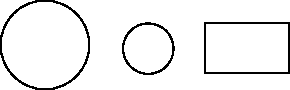
\includegraphics{../graphics/fracPart.pdf}
\]
Explain your reasoning.
\item What fractions could the following picture be illustrating?
\[

\includegraphics{../graphics/whichFrac.pdf}
\]
Explain your reasoning.
\item When Jesse was asked what the $7$ in the fraction $\frac{3}{7}$
  means, Jesse said that the ``$7$'' is the \textit{whole}. Explain
  why this is not completely correct. What is a better description of
  what the ``$7$'' in the fraction $\frac{3}{7}$ means?

\item Find yourself a sheet of paper. Now, suppose that this sheet of
  paper is actually $4/5$ of some imaginary larger sheet of
  paper. 
\begin{itemize}
\item Shade your sheet of paper so that $3/5$ of the larger
  (imaginary) sheet of paper is shaded in. Explain why your shading is
  correct.
\item Explain how this shows that 
\[
\frac{3/5}{4/5} = \frac{3}{4}.
\]
\end{itemize}
\item Try to find the largest rational number smaller than $3/7$.
  Explain your solution or explain why this cannot be done.
\item How many rational numbers are there between $3/4$ and $4/7$?
  Find $3$ of them. Explain your reasoning.
\item A youthful Bart loved to eat hamburgers. He ate $5/8$ pounds of
  hamburger meat a day. After testing revealed that his blood
  consisted mostly of cholesterol, Bart decided to alter his eating
  habits by cutting his hamburger consumption by $3/4$. How many
  pounds of hamburger a day did Bart eat on his new
  ``low-cholesterol'' diet?  Explain your reasoning.
\item A baseball coach once asked me the following question: If a
  pitcher can throw a 90 mph pitch during a game, but can only
  sustain a 60 mph pitch during practice, how close should the pitcher
  stand during practice to ensure that the amount of time it takes the
  ball to reach home plate is the same in practice as it is in the
  game? Explain your reasoning.
\item Courtney and Paolo are eating popcorn. Unfortunately, $1/3$rd of
  the popcorn is poisoned. If Courtney eats $5/16$th of the bowl and
  Paolo eats $5/13$ths of the bowl, did at least one of them eat
  poisoned kernel? Also, at least how many kernels of popcorn are in
  the bowl? Explain your reasoning.
\item Three brothers and a sister won the lottery together and plan to
  share it equally. If the brothers alone had shared the money, then
  they would have increased the amount they each received by \$20. How
  much was won in the lottery? Explain your reasoning.
\item Chris is working on his Fiat. His car's cooling system holds 6
  quarts of coolant, but it is currently 1 quart low. A car should be
  filled with a 50/50 mix of antifreeze and water. Chris accidentally
  added a 25/75 mix, 25 parts antifreeze, and 75 parts water.  How
  much coolant does he have to remove from the cooling system to then
  add 100 percent antifreeze to restore his desired 50/50 mix? Explain
  your reasoning.
\item Best of clocks, how much of the day is past if there remains
  twice two-thirds of what is gone? Explain what this strange question
  is asking and answer the question being sure to explain your
  reasoning---note this is an old problem from the \textit{Greek
    Anthology} compiled by Metrodorus around the year 500.
\item Monica, Tessa, and Jim are grading papers. If it would take
  Monica $2$ hours to grade them all by herself, Tessa $3$ hours to
  grade them all by herself, and Jim $4$ hours to grade them all by
  himself how long would it take them to grade the exams if they all
  work together? Explain your reasoning.
\item Say quickly, friend, in what portion of a day will four
  fountains, being let loose together, fill a container which would
  be filled by the individual fountains in one day, half a day, a
  third of a day, and a sixth of a day respectively? Explain your
  reasoning---note this is an old problem from the Indian text
  \textit{Lilavati} written in the 1200s.
\item John spent a fifth of his life as a boy growing up, another
  one-sixth of his life in college, one-half of his life as a bookie,
  and has spent the last six years in prison. How old is John now?
  Explain your reasoning
\item Diophantus was a boy for $1/6$th of his life, his beard grew
  after $1/12$ more, he married after $1/7$th more, and a son was born
  five years after his marriage. Alas! After attaining the measure of
  half his father's full life, chill fate took the child. Diophantus
  spent the last four years of his life consoling his grief through
  mathematics. How old was Diophantus when he died?  Explain your
  reasoning---note this is an old problem from the \textit{Greek
    Anthology} compiled by Metrodorus around the year 500.
\item Wandering around my home town (perhaps trying to find my former
  self!), I suddenly realized that I had been in my job for
  one-quarter of my life. Perhaps the melancholia was getting the best
  of me, but I wondered: How long would it be until I had been in my
  job for one-third of my life? Explain your reasoning.
\item In a certain adult condominium complex, $2/3$ of the men are
  married to $3/5$ of the women. Assuming that men are only married to
  women (and vice versa), and that married residents' spouses are also
  residents, what portion of the residents are married? 
\begin{enumerate}
\item Before any computations are done, use common sense to guess the
  solution to this problem.
\item Try to get a feel for this problem by choosing numbers for the
  unknowns and doing some calculations. What do these calculations say
  about your guess?
\item Use algebra to solve the problem.
\end{enumerate}
Explain your reasoning in each step above.
\item Fred and Frank are two fitness fanatics on a run from $A$ to
  $B$. Fred runs half the way and walks the other half. Frank runs for
  half the time and walks for the other half. They both run at the
  same speed and they both walk at the same speed. Who finishes first?
\begin{enumerate}
\item Before any computations are done, use common sense to guess the
  solution to this problem.
\item Try to get a feel for this problem by choosing numbers for the
  unknowns and doing some calculations. What do these calculations say
  about your guess?
\item Use algebra to solve the problem.
\end{enumerate}
Explain your reasoning in each step above.
\item Andy and Sandy run a race of a certain distance. Sandy finishes
  $1/10$ of the distance ahead of Andy. After some discussion, Andy
  and Sandy decide to race the certain distance again, this time Sandy
  will start $1/10$ of the distance behind Andy to ``even-up'' the
  competition. Who wins this time?
\begin{enumerate}
\item Before any computations are done, use common sense to guess the
  solution to this problem.
\item Try to get a feel for this problem by choosing numbers for the
  unknowns and doing some calculations. What do these calculations say
  about your guess?
\item Use algebra to solve the problem.
\end{enumerate}
Explain your reasoning in each step above.
\item You have two beakers, one that contains water and another that
  contains an equal amount of oil. A certain amount of water is
  transferred to the oil and thoroughly mixed. Immediately, the same
  amount of the mixture is transferred back to the water. Is there now
  more water in the oil or is there more oil in the water?
\begin{enumerate}
\item Before any computations are done, use common sense to guess the
  solution to this problem.
\item Try to get a feel for this problem by choosing numbers for the
  unknowns and doing some calculations. What do these calculations say
  about your guess?
\item Use algebra to solve the problem.
\end{enumerate}
Explain your reasoning in each step above.
\item While on a backpacking trip Lisa hiked five hours, first along a
  level path, then up a hill, then turned round and hiked back to her
  base camp along the same route. She walks $4$ miles per hour on a
  level trail, $3$ uphill, and $6$ downhill. Find the total distance
  traveled. Explain your reasoning.
\item Three drops of \textit{Monica's XXX Hot Sauce} were mixed with
  five cups of chili mix to make a spicy treat---the hot sauce is much
  hotter than the chili. Later, two drops of \textit{Monica's XXX Hot
    Sauce} were mixed with three cups of chili. Which mixture is
  hotter? Josh suggested the following method to compare the
  concentrations:
\begin{itemize}
\item Remove the second (recipe) from the first, that is: Start with 3
  drops of hot sauce and 5 cups of chili, and remove 2 drops and 3
  cups. So we are now comparing
\[
\text{1 drop and 2 cups}\qquad\text{with}\qquad\text{2 drops and 3 cups.}
\]
\item Now remove the first from the second, that is: Start with 2
  drops and 3 cups, and remove 1 drop and 2 cups. So we are now
  comparing
\[
\text{1 drop and 2 cups}\qquad\text{with}\qquad\text{1 drop and 1
  cup.}
\]
\end{itemize}
Now you can see that the second is more concentrated (and hence
hotter!) than the first. Is this correct? Will this strategy
always/ever work? Explain your reasoning.
\item Let $a$, $b$, $c$, and $d$ be positive integers such that 
\[
a<b<c<d
\]
Is it true that 
\[
\frac{a}{b}<\frac{c}{d}?
\]
Explain your reasoning.
\item\label{P:CF1} Let $a$, $b$, $c$, and $d$ be positive consecutive
  integers such that
\[
a<b<c<d.
\]
Is it true that 
\[
\frac{a}{b}<\frac{c}{d}?
\]
Explain your reasoning.
\item\label{P:CF2} Let $a$, $b$, $c$, and $d$ be positive consecutive
  integers such that
\[
a<b<c<d.
\]
Is it true that 
\[
\frac{a}{b}<\frac{b}{c}<\frac{c}{d}?
\]
Explain your reasoning.
\item Can you generalize Problem \ref{P:CF1} and Problem \ref{P:CF2}
  above? Explain your reasoning.
\item Let $a$, $b$, $c$, and $d$ be positive integers such that 
\[
\frac{a}{b}<\frac{c}{d}.
\]
Is it true that 
\[
\frac{a}{a+b}<\frac{c}{c+d}?
\]
Explain your reasoning.
\end{enumerate}
\end{problems}

\section{Decimal Representations}
Text

\begin{activitynote}
Activities \ref{A:DecNotNice} and \ref{A:Shampoo} complement this section well. 
%% Decimals Aren't So Nice & Shampoo, Rinse, ... 
\end{activitynote}

\section{Ratios and Proportional Relationships}
Text

\begin{activitynote}
Activities \ref{A:Ratios} through \ref{A:ProblemSolved} complement this section well. 
%% Poor Old Horatio
%% Ratio Oddities
%% Problem Solved
As a conclusion, we suggest doing Activity \ref{A:dreadedStoryProblem}.
\end{activitynote}

\begin{activitynote}
\end{activitynote}

\section{Functions and Beyond}
Text
\begin{activitynote}
Activity \ref{A:walk} complements this section well.   % Walk the Line
\end{activitynote}

\begin{activitynote}
This is a good point to do activities \ref{A:doesntAddUp} through \ref{A:billy}. 
%% Something Doesn't Add Up
%% Gertrude the Gumchewer
%% Billy the Bouncing Ball 
\end{activitynote}

\subsection{Rules and Meanings of Exponents}
Text





